\section{Design}
\label{sec:design}

This section presents the design of {\name}, including the overall architecture,
the data model, and the protocols for the {\em put}, {\em get}, and {\em delete} operations.

\subsection{Overview and Challenges}

\begin{figure}[tp]
\centering
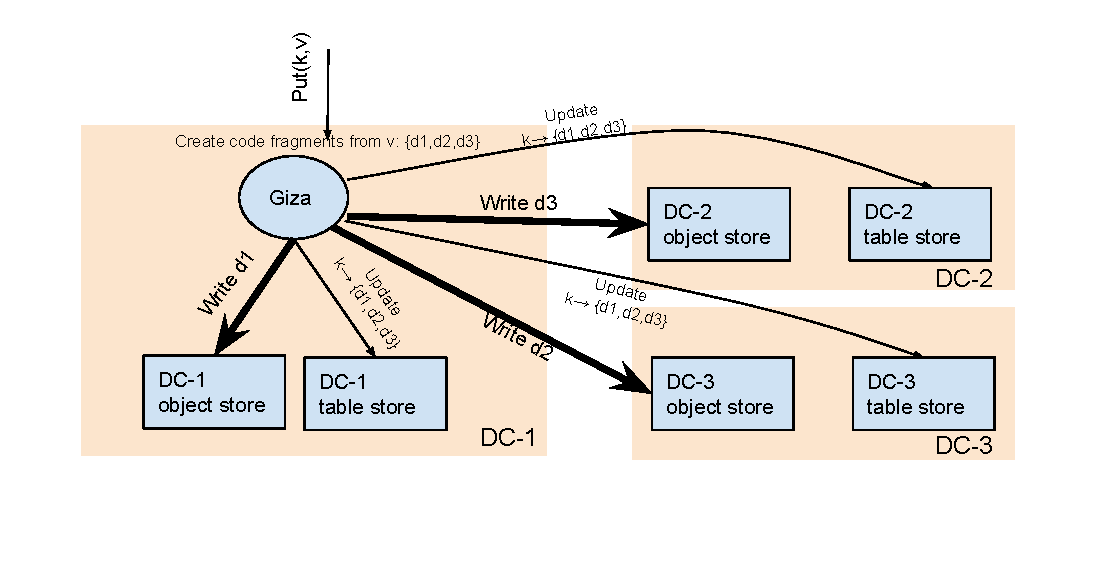
\includegraphics[width=0.52\textwidth]{fig/Giza}
\caption{Giza architecture\label{fig:arch}}
\end{figure}

\paragraph{Architecture}
{\name} is a global-scale cloud storage system that spans across many data
centers. It stores mutable, versioned objects. Figure~\ref{fig:arch} shows the
architecture of \name. \name stores an object through a {\em put} operation, consisting of a data operation and a metadata operation. These operations are executed in parallel to improve performance. On the data path, \name splits and
encodes the object into data and parity fragments.
Each coded fragment is named by a unique identifier and stored in a different DC.
Each update to the object creates a new version. The version
numbers and the coded fragment IDs in each version constitutes the
metadata of the object. On the metadata path, \name replicates the metadata
across the data centers.

\name is implemented on top of the existing Azure Storage infrastructure.
It stores the coded fragments in Azure Blob storage 
and the metadata in Azure Table storage.
This provides two advantages. First, doing so allows the rapid development of \name
by re-using mature, deployed, and well-tested systems. Second, it simplifies the
failure recovery and deployment: \name runs on stateless nodes and can be readily
integrated with the rest of the stateless cloud storage front-ends.

\paragraph{Technical challenges}
In \name, each coded fragment is named by a unique identifier.
As a result, fragments are immutable, which simplifies the data path.

The metadata path is more tricky, facing three main technical challenges:
\begin{enumerate}

\item {\it Building a strongly consistent, 
geo-replicated metadata store out of existing single-DC cloud tables.}
\name runs on stateless nodes and leverages existing well-tested
cloud storage infrastructure to persist all data and metadata.
The architecture simplifies development, deployment, and operation.
This makes Giza quite different from other systems
operating stateful servers (e.g., Cassandra, Megastore, Spanner, etc.).
In addition, the cloud tables only guarantee consistency within single data center.
Giza needs to orchestrate a collection of individual cloud tables across multiple data centers
and achieve strong consistency globally.

\item {\it Jointly optimizing the data and metadata paths to achieve a single
  cross-DC round trip for read/write operations.}
Most existing systems employ a primary-based approach,
which incurs extra cross-DC round trip for secondary data centers.
\name, on the other hand, is leaderless and
combines the data and metadata path in such a way that achieves
	single cross-DC round trips for both read and write from any data center.
	\comment{
	A naive approach would execute
  the data and metadata path sequentially: 
	first writes the coded fragments and completes the data path, 
	and then completes the metadata path. Doing so guarantees that
  the metadata written and externally visible always matches with the stored
  data. However, each write operation will require at least two cross-DC round
  trips. Similarly, a naive approach for read operation would take the first
  cross-DC round trip to retrieve the metadata and then the second round trip to
  retrieve the data. \name combines the data and metadata path and achieves
	a single cross-DC round trip for both read and write.
	}

\item {\it Performing garbage collection efficiently and promptly.} When a data
  object is deleted or its old versions are garbage collected, \name must
  remove obsolete fragments and/or metadata from the underlying cloud blob
	and table storage.
	%\name must also remove fragments generated by a failed data path write.
	This turns out to be non-trivial because \name's
  garbage collection mechanism must be able to handle data center failures while
  ensuring data consistency and durability.

\end{enumerate}

\subsection{Paxos using Cloud APIs}

To address the above challenges, Giza adapts well-known distributed algorithms
- Paxos and Fast Paxos - in a novel way on top of Azure Table.

\subsubsection{Paxos and Fast Paxos in Giza: A Brief Primer}

The Paxos algorithm~\cite{lamport01paxos} provides a mechanism to reach
consensus among a set of {\em acceptors} and one or more {\em proposers}.
A proposer initiates a Paxos voting process by first picking a distinguished {\em
  ballot}. All ballots are unique and can be compared to each other. The
proposer sends requests and proposed values to the acceptors.
Each acceptor decides whether to accept a request based on its
own state. A proposed value is {\em committed} when it is accepted by a {\em
  quorum} of the acceptors. The acceptors update their states when a request or
value is accepted.

Paxos is typically implemented via active acceptors, which are
capable of comparing the ballot of incoming requests with their own states and
deciding whether to accept the requests.
\name works differently and uses the cloud tables as the acceptors.
It implements the acceptor logic leveraging Azure Table's {\em atomic conditional update} capability.

Paxos takes two {\em phases} to reach consensus, where {\em phase} $1$ prepares
a ballot and {\em phase} $2$ commits a value. Since each phase takes one round
trip, applying Paxos in Giza results in two cross-DC round trips for the metadata path.

%writes~\footnote{Typical Paxos optimization elects a distinguished leader. The
  %leader executes {\em phase} $1$ in advance and only takes one round trip in
  %{\em phase} $2$ to reach consensus. This, however, requires relaying all
  %updates through the leader. In the cross-DC scenario, it takes one cross-DC
  %round trip to relay updates originating from non-leader DCs. Therefore, these
  %updates still take two cross-DC round trips to commit.}.

Fast Paxos~\cite{lamport05fast} is a variation of Paxos that optimizes the
performance over cross-DC acceptors. It employs two types of rounds: fast round
and classic round. A fast round sends a PreAccept request and takes a single
round trip to commit a value. A classic round resembles the two phases in Paxos
and takes two round trips. The fast round in Fast Paxos requires a larger quorum.
With $3$ acceptors,
a value is committed only when it is accepted by all the 3 acceptors (quorum size of 3).
In comparison, Paxos is able to commit the value with 2 out of the 3 acceptors (quorum size of 2).
The advantage of Fast Paxos is that when all the 3 acceptors respond, the value is committed
in a single round trip. The requirement of larger quorum fits \name perfectly,
as Giza data path already requires storing fragments in 3 or more data centers.

Giza implements both Paxos and Fast Paxos. This paper discusses Fast Paxos only as
its implementation requires more care (but achieves lower latency) than Paxos.

\begin{figure}[tp]
\centering
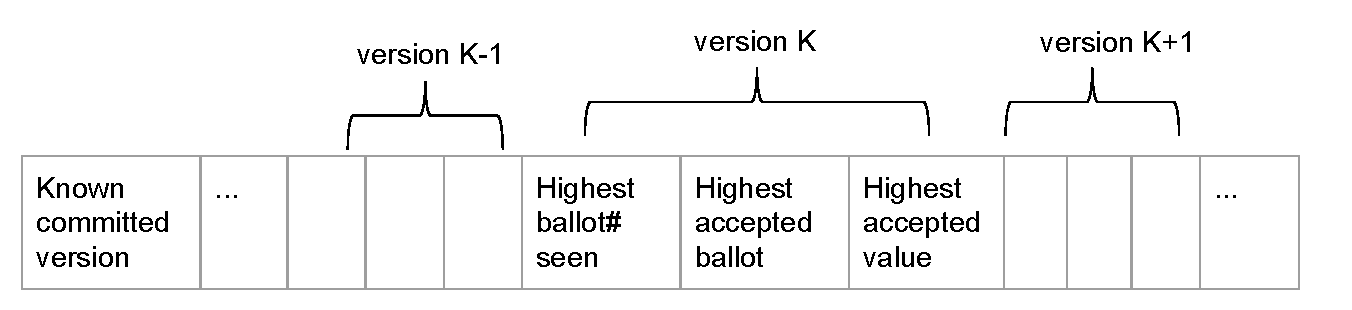
\includegraphics[width=0.5\textwidth]{fig/Giza_Metadata}
\caption{For each object, \name stores the Paxos protocol state and the object metadata 
in a single row in the underlying cloud table.\label{fig:metadataschema}}
\end{figure}

\subsubsection{Metadata Storage Layout}

\name needs to persist the Paxos states together with the metadata for an object in the cloud table. 
We use one table row per object, with a dynamic number of columns,
where each version of the object takes three columns. The layout of each table row is
shown in Figure~\ref{fig:metadataschema}.

Each version is represented by a consecutive natural numbers, starting
from $1$. Every \name write to the object creates a new version. For each
version, \name initiates a separate Paxos instance and uses Paxos to guard
against races from concurrent writes and cloud table failures.
The metadata of all versions and the states of all the Paxos instances
are stored in the same table row. Specifically, the metadata contains a triplet
of columns for each version (Figure~\ref{fig:metadataschema}). Two
of the columns are Paxos states: {\tt highest ballot seen} and {\tt highest accepted
  ballot}. The other column, {\tt highest accepted value}, stores the metadata,
including the erasure coding scheme, the unique fragment IDs,
and which DCs the fragments are stored at.

{\name} additionally maintains a set of {\tt known committed versions} for all
those that have been successfully committed. This is to facilitate both {\em put}
and {\em get} operations, as discussed in the following sections.

\subsubsection{Metadata Write - Common Case}

The metadata path begins by choosing a proper new version number to initiate a 
Fast Paxos instance. Since version numbers need to be consecutive, 
the new version should succeed the most recently committed version.
{\name} identifies a proper version number in an optimistic fashion.
Specifically, it reads {\tt known committed versions} from the table in its local DC,
then uses the next higher number as the new version number.
In the uncommon case that the newly chosen version number has already been committed
(but this DC missed the corresponding commit), the commit attempt would fail.
Through the process, Giza learns the committed versions from the remote DCs,
which allows it to choose a correct version number for retry.

Following Fast Paxos, Giza sends a PreAccept request to all the cloud tables,
each located in a different DC. 
Each request is an {\em atomic conditional update} on the table row of the object.
If there are no competing writes of the same object, the PreAccept request
will succeed in updating the table row. Otherwise, the PreAccept request will be
rejected by the table and leave the table row unchanged. 

Whenever {\name} receives a {\em fast quorum} of positive PreAccept
responses, the corresponding version is considered to have been committed.
{\name} asynchronously sends a Commit confirmation to all the cloud tables
to update the set of {\tt known committed versions} to include the recently
committed version. The Commit confirmation is again an atomic conditional
update, which only succeeds if the version number is not yet included in the
current set.

Since the Commit confirmation is completed asynchronously, the critical path
only involves the PreAccept request and response. Hence, without conflict, the
above described metadata write involves only one cross-DC round trip and is
referred to as the {\em fast path}.

\subsubsection{Metadata Write with Contention}

The fast path may fail when {\name} fails to collect a fast quorum of
positive PreAccept responses. This may result from concurrent updates to the
same object (contention), or because one or more cloud tables fail. In this
case, {\name} enters what is referred to as a \emph{slow path} to perform
classic Paxos in order to guarantee safety.

On the slow path, {\name} first picks a distinguished ballot number and
then replicates a Prepare request to write the ballot to all the metadata tables
and wait for a majority of responses. The Prepare request is an atomic conditional
update operation. The operation succeeds only if the {\tt highest ballot seen}
is no more than the ballot in the Prepare request. The operation also returns
the entire row as a result.

Upon collecting a majority of successful replies, {\name} needs to pick
a value to commit. The rule for picking the value is categorized into three
cases. In case 1, Giza looks for the highest accepted ballot in the replies. If
there is one, the value from the reply is picked. In case 2, the replies contain
no accepted value, but rather pre-accepted values. Giza picks the pre-accepted
value returned by the maximum responses in the quorum. Both case 1 and 2
imply the possibility of an ongoing Paxos instance, so Giza picks the value so
as to complete the Paxos instance first. It then starts with a new version and
follows the fast path to commit its current metadata. In case 3, there is
neither pre-accepted nor accepted value, which implies no real impact from
contention. Giza picks its current metadata as the value and proceeds to the next
steps.

% JinL: my understanding is that Azure Table's conditional update is based on etag. 
% That is, the conditional update is performed if old_etag = cur_etag, and is rejected otehrwise. 
% It can't perform a function to check whether {\tt highest ballot seen} and/or {\tt highest accepted ballot} 
% is alrger. 
Once {\name} picks the value, it replicates an Accept request to all the
metadata tables. The accept request is again an atomic conditional update; it
succeeds in writing {\tt highest accepted ballot} and {\tt highest accepted
  value} if neither {\tt highest ballot seen} nor {\tt highest accepted ballot}
is larger. 
As soon as a majority of Accept requests succeed, \name considers
the corresponding metadata write completed and sends acknowledgment to clients. 
Additionally, a Commit confirmation is replicated in the background, as
described before.

\subsubsection{Metadata Read}

To get the metadata of the \emph{latest} object version, it is {\em insufficient} for
\name to only read the corresponding metadata table row from its local DC. This
is because the local DC might not be part of the majority quorum that has
accepted the latest version. To ensure correctness, Giza needs to read the
metadata rows from more than one DC.

In the common case, {\tt known committed versions} is up-to-date and
includes the latest committed version (say version $k$).
Giza reads version $k$ from the metadata table row in a local DC.
It then confirms the lack of higher committed versions than $k$,
from the metadata table row in a non-local DC.
Hence, in the case that the metadata is replicated to 3 DCs, 
the metadata from 2 DCs (one local and one non-local) 
leads to a decisive conclusion that version $k$ is the
latest committed version. It is therefore safe for \name to return
version $k$ to clients.

In general, \name reads the metadata table rows from all the DCs.
Whenever a majority rows have matching {\tt known committed versions} and have
not accepted any value for a higher version, \name returns the metadata
of the highest committed version.

If the replies contain an accepted value with a higher version number than the
{\tt known committed versions}, \name needs to follow a slow path
similar to the one in the write operation. This is to confirm whether the higher
version has indeed been committed.

% continue to design_part2.tex
